\section[Introdução]{Introdução}

O projeto Informativo para Imigrantes e Refugiados teve como objetivo principal desenvolver um aplicativo mobile para facilitar o acesso à informação para pessoas imigrantes e refugiadas. Os stakeholders Éfren Alvarado, Alex Guilherme e Henrique trouxeram como problema a dificuldade que esse público enfrenta para encontrar informações confiáveis sobre direitos, oportunidades de educação e programas de acolhimento disponíveis no Brasil.

A proposta do aplicativo é reunir essas informações em um único lugar, permitindo que 
\ac{ong}s, universidades, escolas e outras instituições cadastrassem programas com detalhes suficientes para orientar melhor os usuários. Dessa forma, o produto buscava reduzir a barreira de acesso à informação e apoiar a integração social e educacional de imigrantes e refugiados.

O projeto foi desenvolvido durante o segundo semestre de 2023, com início em 4 de agosto de 2023 e conclusão em 8 de dezembro de 2023, sob orientação do professor Dilnei Venturini. A Figura~\ref{fig:ages-i-time} registrou o time envolvido no projeto.

\begin{figure}[H]
    \centering
    \small
    \caption{Time do projeto Informativo para Imigrantes e Refugiados}
    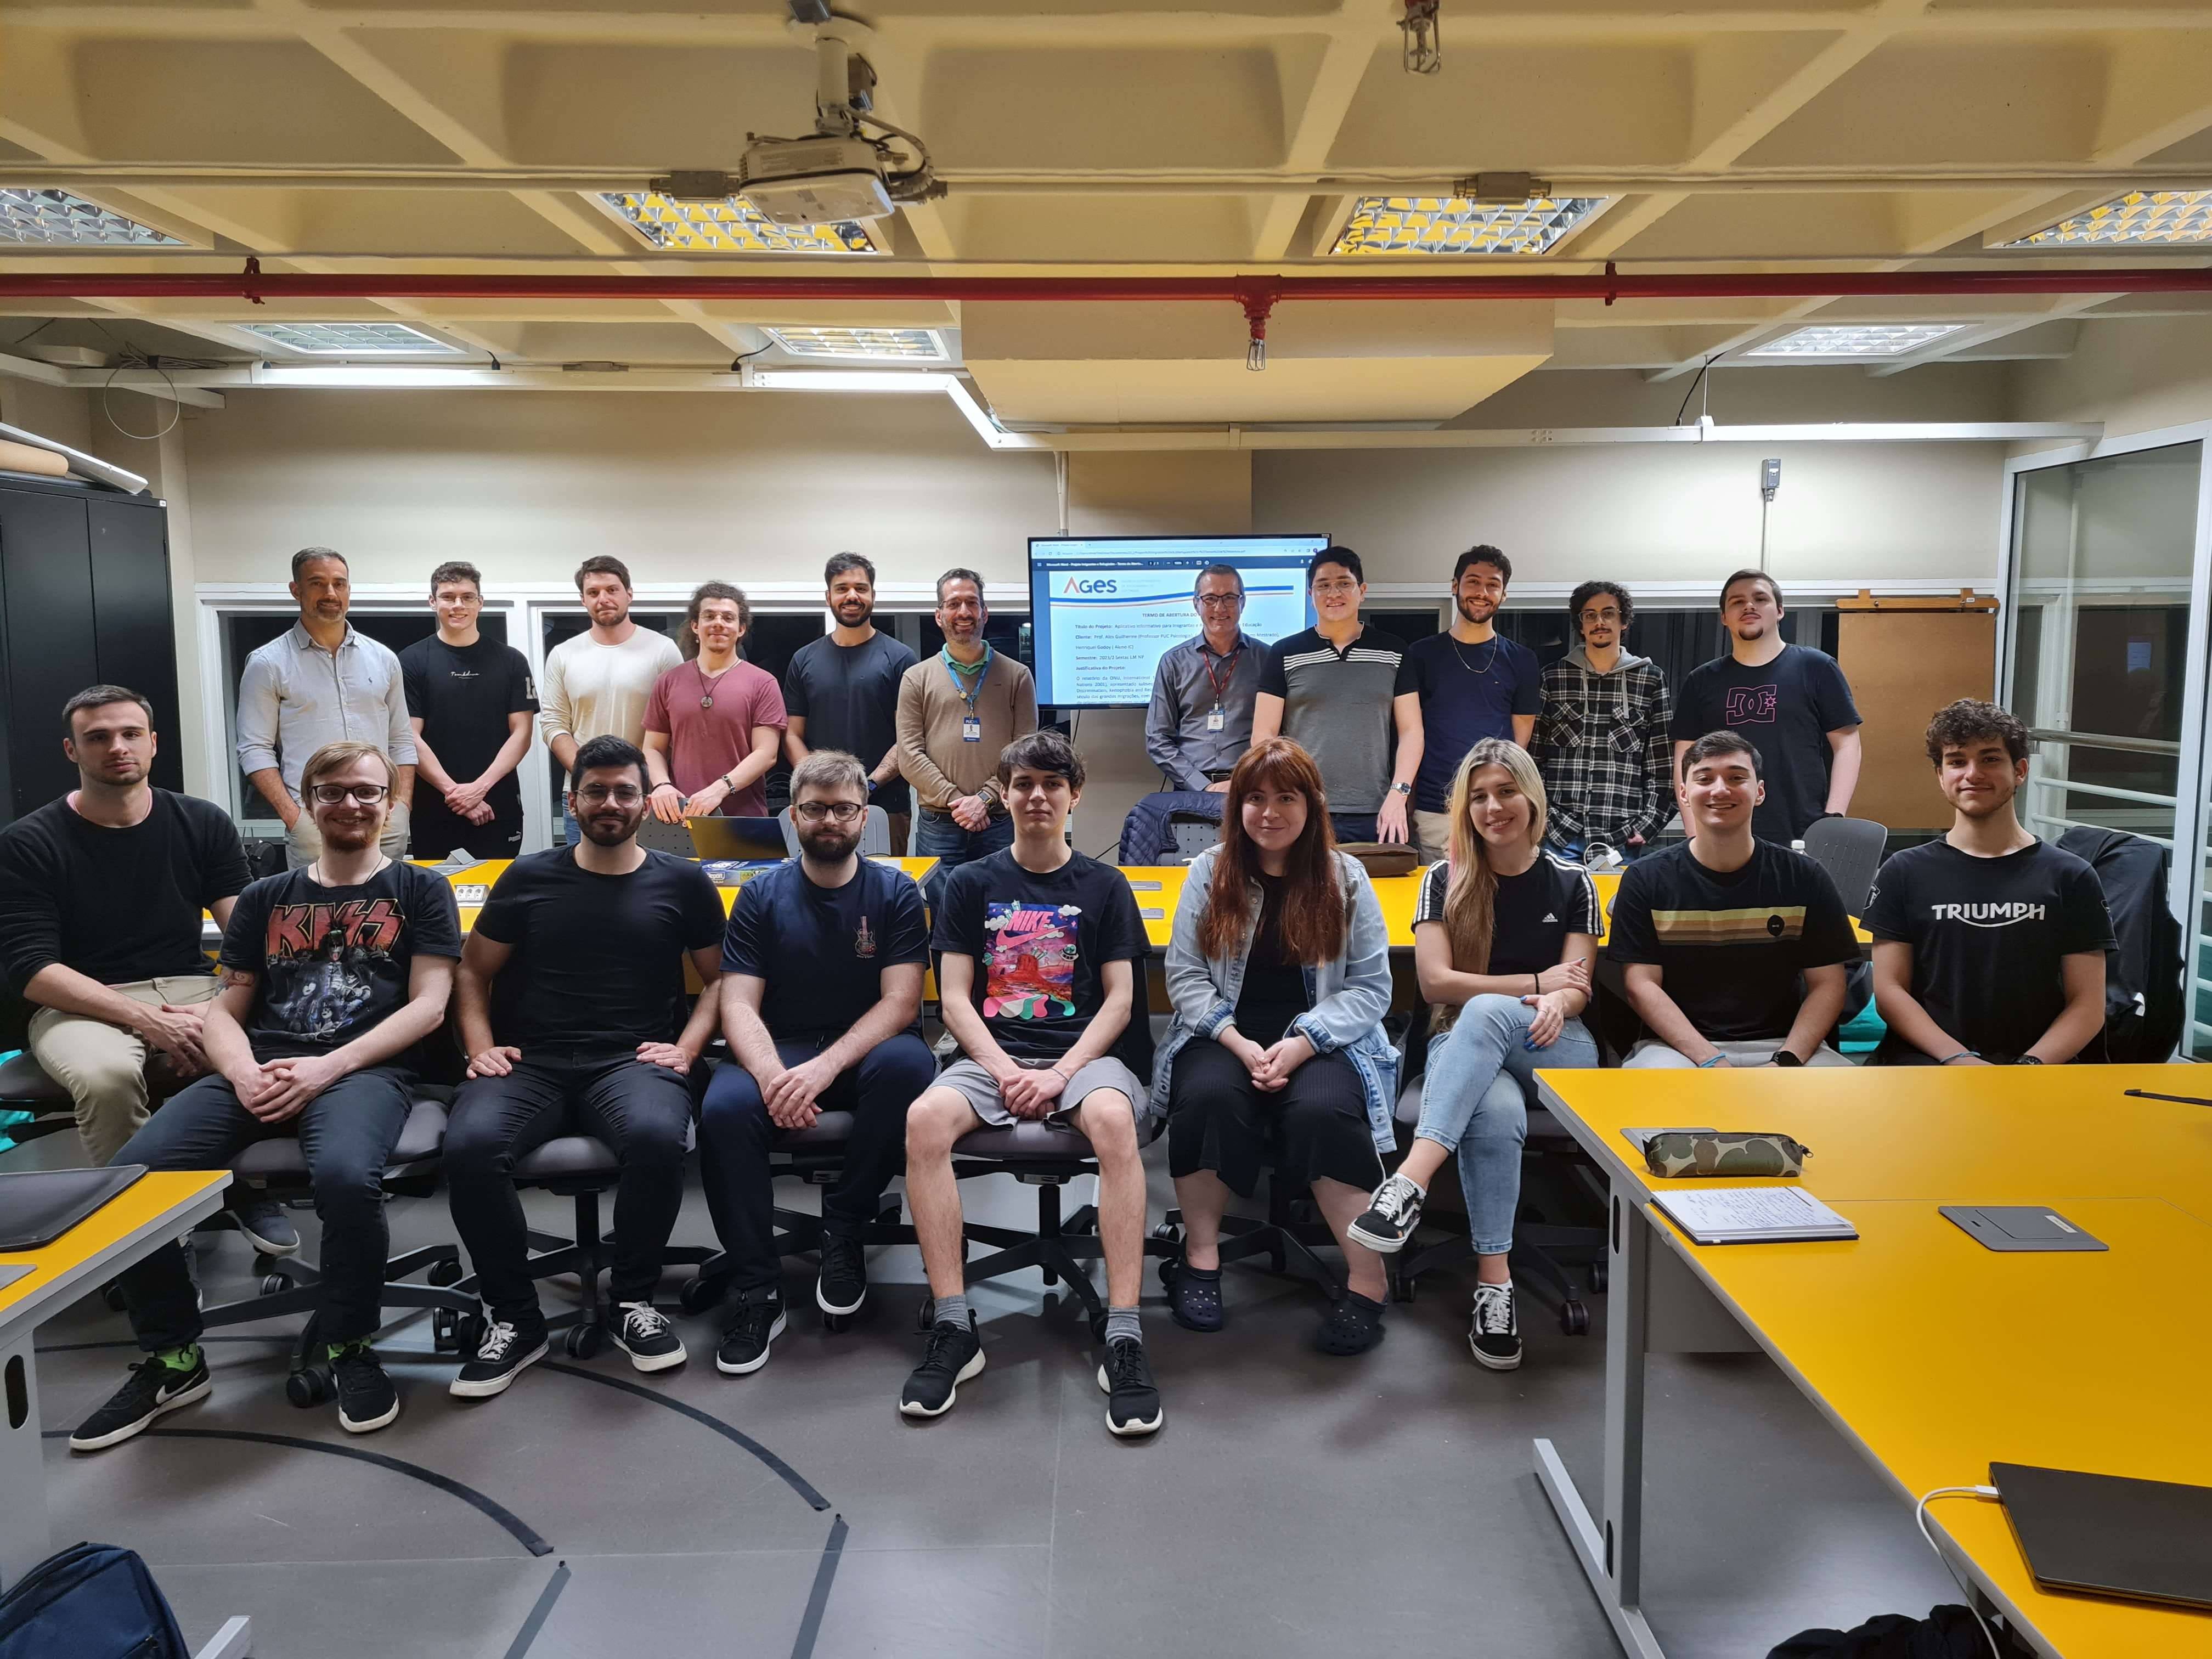
\includegraphics[width=1\linewidth]{conteudo//2 - ages I//conteudo//figures/fototime.jpg}
    Fonte: wiki do projeto
    \label{fig:ages-i-time}
\end{figure}
